%
% Frame 1
%
\begin{frame}[t]{Remaining Work}
\vspace{-3ex}
\begin{center}
\only<1>{\hh{First Order Logic} \hspace{10ex} \hh{Lexical Methods} \\}
\only<1>{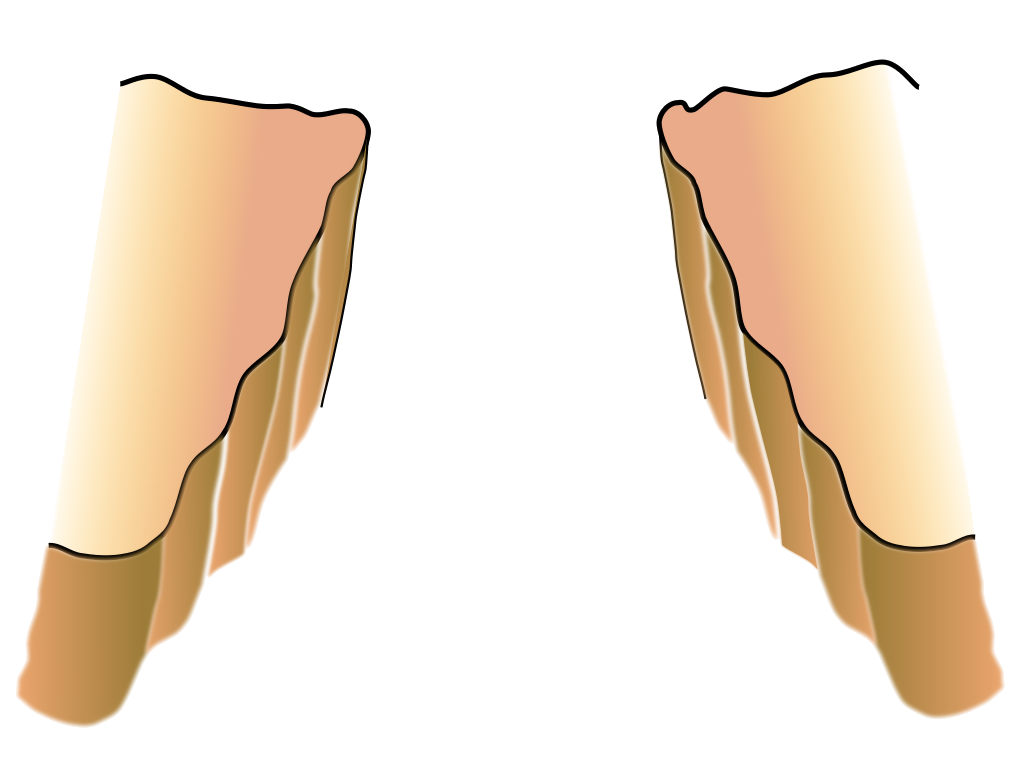
\includegraphics[height=4cm]{../img/chasm.png}}

\only<2->{\hh{Natural Logic} \hspace{3ex} \hh{Lexical Methods} \\}
\only<2->{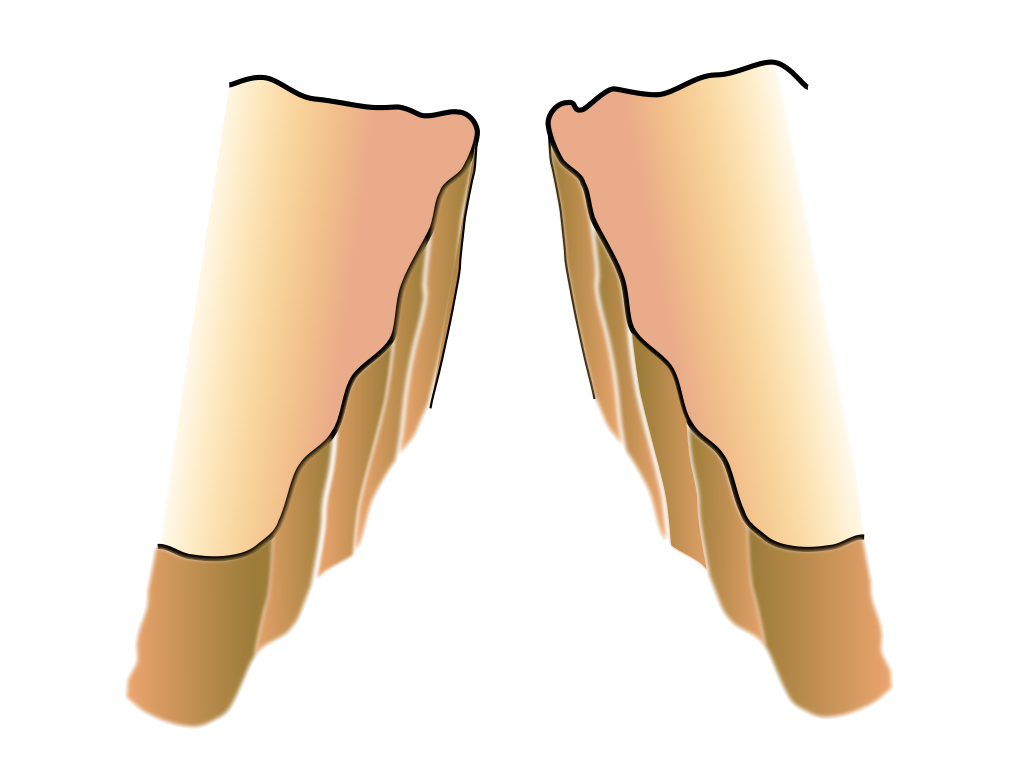
\includegraphics[height=4cm]{../img/chasm-close.png}}
\end{center}
\pause
\pause

\begin{itemize}
\item Already useful for textual entailment 
      \cite{key:2008maccartney-natlog,key:2009maccartney-thesis}
\pause
\item \hh{This thesis:} Useful for question answering \newline
      \hh{This thesis:} We can bridge the two methods
\end{itemize}

\only<4->{
\begin{textblock*}{5cm}(4.5cm,3.5cm)
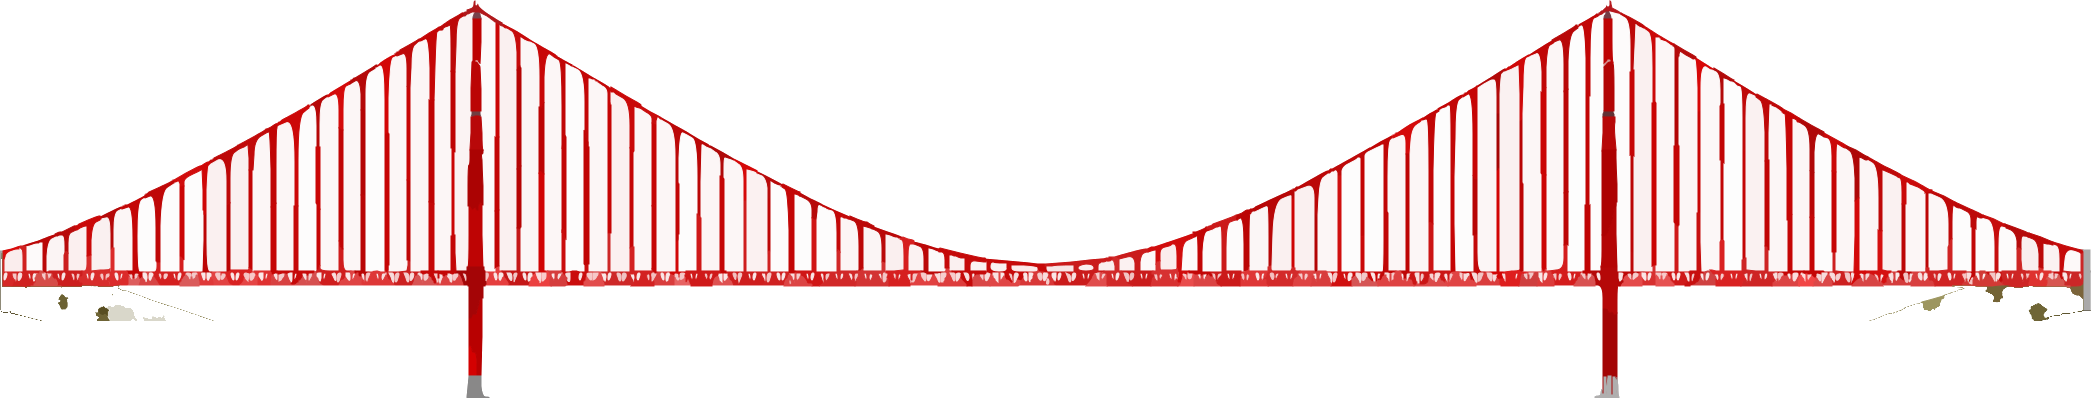
\includegraphics[width=4cm]{../img/golden-gate.png}
\end{textblock*}
}

\end{frame}

%
% Frame 2
%
\begin{frame}[noframenumbering]{Remaining Work}
\begin{center}
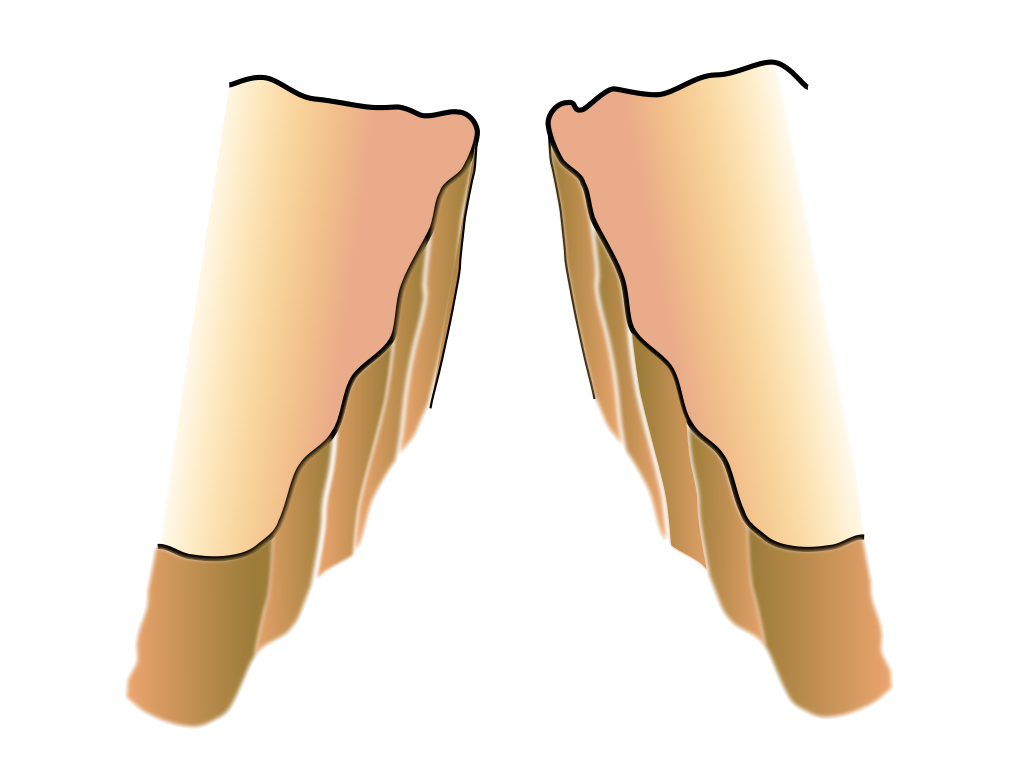
\includegraphics[height=2cm]{../img/chasm-close.png}
\end{center}
\vspace{-2ex}


\begin{enumerate}
\item Encode logic in traditionally lexical representations
  \cite{key:2013bowman-natlog,key:2015bowman-natlog}
\pause
\item Make natural logic more expressive
\pause
\begin{itemize}
  \item Propositional + Natural logics: \\
       \hspace{2ex}\w{Apples are red} $\lor$ \w{\textcolor<4->{darkred}{Bananas are red}} \\
       \hspace{2ex}\w{\textcolor<4->{darkred}{Bananas are not red}} \\
       \hspace{0ex}$\therefore$ \w{Apples are red}
  \pause
  \pause
  \item Syntactic and idiomatic entailment models: SNLI corpus?
\end{itemize}
\end{enumerate}
\end{frame}
